\documentclass[presentation]{beamer}
\mode<presentation>{\usetheme{AMSBolognaFCrev}}

\usepackage[utf8]{inputenc}
\usepackage[T1]{fontenc}
\usepackage{booktabs}
\usepackage{array}
\usepackage{tabularx}
\usepackage{tikz}
\usepackage[ddmmyyyy]{datetime}
\usepackage[export]{adjustbox}
\usetikzlibrary{arrows.meta,positioning,shapes.geometric,fit,calc}

\renewcommand{\dateseparator}{/}
\newcommand{\sectiontitleframe}[1]{
\begin{frame}[plain,c]
\begin{center}
{\usebeamerfont{title}\usebeamercolor[fg]{title}#1}
\end{center}
\end{frame}
}

\tikzset{
    opsbox/.style={draw, rounded corners, align=center, font=\scriptsize,
        minimum height=0.72cm, text width=2.15cm},
    smallopsbox/.style={draw, rounded corners, align=center, font=\tiny,
        minimum height=0.55cm, text width=1.65cm},
    opsarrow/.style={-{Stealth[length=2mm]}, thick}
}

\title[Lesson 9]{Operational Security and Incident Response}
\institute[Data Privacy and Security]{Healthcare Data Privacy and Security}
\author[\sspeaker{G. Pisano}]{\speaker{Giuseppe Pisano} \\\href{mailto:g.pisano@unibo.it}{g.pisano@unibo.it}}
\date[August, 2026]{August, 2026}
%
\titlegraphic{
\begin{center}
    
\includegraphics[width=0.35\textwidth, valign=c]{logos/intestazione.png}
    
\includegraphics[width=0.16\textwidth, valign=c]{logos/unibo_logo_2.png}
    
\includegraphics[width=0.11\textwidth, valign=c]{logos/makeni_logo_2.png}
    
\includegraphics[width=0.20\textwidth, valign=c]{logos/cuamm_logo_png.png}
\end{center}
\centering
\tiny{S.K.I.L.L.E.D --- AID013244/04/2\\Strategic Knowledge and Inclusive Lifelong Learning in the health sector for youth Employability and Development}
}

\newcommand{\scenario}{St. Isidore Hospital}
\newcommand{\takeawaysframe}[2]{
\begin{frame}[c]{Recap: \insertsection}
\begin{block}{Takeaways}
#1
\end{block}
\begin{exampleblock}{In \scenario}
#2
\end{exampleblock}
\end{frame}
}

\begin{document}

\setbeamertemplate{frametitle}
{
    \nointerlineskip
    \begin{beamercolorbox}[sep=0.3cm,ht=2.2em,wd=\paperwidth]{frametitle}
        \vbox{}\vskip-2ex%
        \strut\insertframetitle\hfill\raisebox{-0.2\height}{
\includegraphics[width=2cm]{logos/cuamm_logo_png.png}}\strut
        \vskip-0.8ex%
    \end{beamercolorbox}
}

\begin{frame}[allowframebreaks]
\titlepage
\end{frame}

\begin{frame}[c,allowframebreaks]{Roadmap}
\tableofcontents[hideallsubsections]
\end{frame}

\begin{frame}[c]{How This Lesson Progresses}
\begin{block}{Learning path}
We turn the previous lessons into operational habits: prevent common incidents, prepare backups,
detect ransomware, contain compromise, recover safely, and communicate clearly.
\end{block}

\begin{exampleblock}{Hospital storyline}
At 07:20 on Monday, \scenario{} discovers that the EHR is unavailable, shared folders are encrypted,
and a nurse reports a suspicious email attachment. The question is no longer theoretical: how does
the hospital keep treating patients?
\end{exampleblock}
\end{frame}

\begin{frame}[c]{Why Operations Close the Course}
\begin{block}{Connection}
Security controls only matter if they survive real work. Ransomware, scams, misconfiguration, lost
devices, and vendor failures test whether authentication, access control, encryption, networking,
logging, backups, and privacy governance were implemented as a system.
\end{block}

\begin{exampleblock}{Running example}
A strong password policy helps before the incident. Network segmentation helps during the incident.
Backups determine recovery. Privacy governance shapes breach notification and patient communication.
\end{exampleblock}
\end{frame}

\section{Operational Security Mindset}
\sectiontitleframe{Operational Security Mindset}

\begin{frame}[c]{Section Context: Operational Security Mindset}
\begin{block}{What we are talking about}
Operational security is the daily practice of keeping systems safe enough to support care. It is
less glamorous than cryptography or firewalls, but many hospital incidents begin with routine
failures: weak passwords, unpatched systems, unclear ownership, and untested backups.
\end{block}

\begin{exampleblock}{Hospital lens}
The hospital does not need perfect security. It needs resilient security: controls that reduce the
chance of incidents and limit harm when incidents still happen.
\end{exampleblock}
\end{frame}

\begin{frame}[c]{From Framework to Action}
\begin{block}{NIST CSF 2.0}
The NIST Cybersecurity Framework organizes cybersecurity outcomes around \textbf{govern},
\textbf{identify}, \textbf{protect}, \textbf{detect}, \textbf{respond}, and \textbf{recover}
\cite{nist_csf}.
\end{block}

\begin{exampleblock}{Running example}
For \scenario{}, governance means assigning owners. Identify means knowing critical systems. Protect
means MFA and segmentation. Detect means logs and alerts. Respond means containment. Recover means
restoring care safely.
\end{exampleblock}
\end{frame}

\begin{frame}[c]{Operational Security Scheme}
\begin{center}
\begin{adjustbox}{max width=\textwidth}
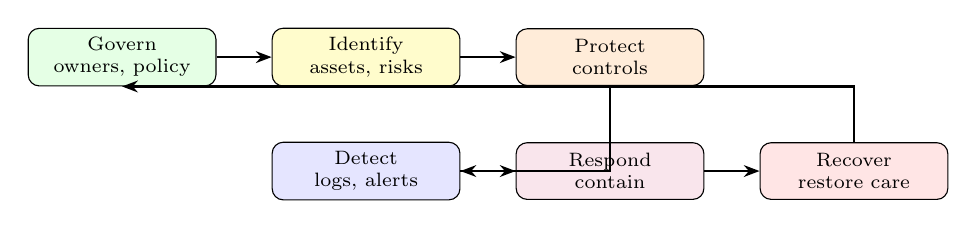
\begin{tikzpicture}[node distance=0.7cm]
\node[opsbox, fill=green!10] (govern) {Govern\\owners, policy};
\node[opsbox, right=of govern, fill=yellow!20] (identify) {Identify\\assets, risks};
\node[opsbox, right=of identify, fill=orange!15] (protect) {Protect\\controls};
\node[opsbox, below=of identify, fill=blue!10] (detect) {Detect\\logs, alerts};
\node[opsbox, right=of detect, fill=purple!10] (respond) {Respond\\contain};
\node[opsbox, right=of respond, fill=red!10] (recover) {Recover\\restore care};
\draw[opsarrow] (govern) -- (identify);
\draw[opsarrow] (identify) -- (protect);
\draw[opsarrow] (protect) |- (detect);
\draw[opsarrow] (detect) -- (respond);
\draw[opsarrow] (respond) -- (recover);
\draw[opsarrow] (recover.north) |- (govern.south);
\end{tikzpicture}
\end{adjustbox}
\end{center}
\end{frame}

\begin{frame}[c]{The Hospital Asset Question}
\begin{block}{Identify first}
You cannot protect what nobody owns or understands. Operational security starts with an inventory:
systems, users, vendors, backups, network paths, data types, dependencies, and critical clinical
workflows.
\end{block}

\begin{exampleblock}{Running example}
If the EHR is down, can the emergency department still see allergies? If the laboratory system is
down, can clinicians still receive urgent results? These are asset and dependency questions.
\end{exampleblock}
\end{frame}

\takeawaysframe{
\begin{itemize}
    \item Operational security turns controls into repeatable work.
    \item Governance and ownership matter as much as tools.
    \item Healthcare resilience starts from clinical dependencies.
\end{itemize}
}{
St. Isidore maps systems by patient-care impact, not only by technical category.
}

\section{Scams, Phishing, and Human Entry Points}
\sectiontitleframe{Scams, Phishing, and Human Entry Points}

\begin{frame}[c]{Section Context: Scams and Phishing}
\begin{block}{What we are talking about}
Many incidents start with social engineering: a person is tricked into opening a file, entering a
password, approving an MFA request, paying a fake invoice, or granting remote access.
\end{block}

\begin{exampleblock}{Hospital lens}
Attackers do not need to defeat encryption if they can convince a busy employee to run malware or
share credentials.
\end{exampleblock}
\end{frame}

\begin{frame}[c]{Common Healthcare Scams}
\small
\begin{tabularx}{\textwidth}{@{}p{0.27\textwidth}X@{}}
\toprule
\textbf{Scam} & \textbf{Hospital example} \\
\midrule
Phishing attachment & ``Updated rota'' spreadsheet installs malware \\
Credential harvesting & fake patient portal login page steals passwords \\
MFA fatigue & repeated push prompts until a user accepts \\
Invoice fraud & supplier bank account change request \\
Fake IT support & caller asks nurse to install remote tool \\
Executive impersonation & urgent request to send patient or payroll file \\
\bottomrule
\end{tabularx}
\end{frame}

\begin{frame}[c]{What Staff Should Notice}
\begin{block}{Red flags}
Unexpected urgency, mismatched sender domains, unusual file types, password requests, links to
login pages, pressure to bypass procedure, and ``keep this confidential'' instructions should slow
the user down.
\end{block}

\begin{exampleblock}{Running example}
A message says: ``Your mailbox is full, login now or lose access before surgery schedule upload.''
The right action is to report it, not to click.
\end{exampleblock}
\end{frame}

\begin{frame}[c]{Make Reporting Easy}
\begin{block}{Operational advice}
Training is not enough if reporting is slow or punitive. Staff need a simple way to report suspicious
emails, calls, files, and logins, and they need feedback that reporting helped.
\end{block}

\begin{exampleblock}{Running example}
\scenario{} adds a report-phishing button and a phone number for urgent suspicious calls. The
security team treats reports as early-warning signals, not as embarrassment.
\end{exampleblock}
\end{frame}

\begin{frame}[c]{Controls That Reduce Social Engineering Impact}
\begin{block}{Defense in depth}
Use MFA, disable macros where possible, filter email, block known malicious domains, limit admin
rights, restrict remote tools, monitor unusual login locations, and require out-of-band verification
for payment or vendor-account changes.
\end{block}

\begin{exampleblock}{Running example}
If a receptionist enters credentials into a fake page, MFA and conditional access may prevent login.
If the attacker still logs in, least privilege limits what the account can access.
\end{exampleblock}
\end{frame}

\takeawaysframe{
\begin{itemize}
    \item Scams target attention, pressure, and routine.
    \item Good reporting is a security control.
    \item Technical controls reduce the blast radius of human mistakes.
\end{itemize}
}{
St. Isidore designs procedures so staff can pause, verify, and report without delaying care.
}

\section{Ransomware}
\sectiontitleframe{Ransomware}

\begin{frame}[c]{Section Context: Ransomware}
\begin{block}{What we are talking about}
Ransomware is an operational crisis: attackers may steal data, encrypt systems, disrupt care, and
pressure the organization through extortion. Hospitals are attractive because downtime can affect
patient safety.
\end{block}

\begin{exampleblock}{Hospital lens}
The ransom note is only the visible symptom. The incident may include credential theft, lateral
movement, backup deletion, data exfiltration, and weeks of recovery work.
\end{exampleblock}
\end{frame}

\begin{frame}[c]{Typical Ransomware Chain}
\begin{center}
\begin{adjustbox}{max width=\textwidth}
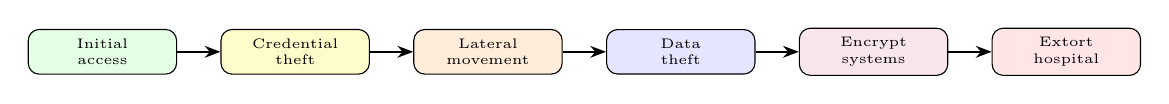
\begin{tikzpicture}[node distance=0.55cm]
\node[smallopsbox, fill=green!10] (entry) {Initial\\access};
\node[smallopsbox, right=of entry, fill=yellow!20] (cred) {Credential\\theft};
\node[smallopsbox, right=of cred, fill=orange!15] (move) {Lateral\\movement};
\node[smallopsbox, right=of move, fill=blue!10] (exfil) {Data\\theft};
\node[smallopsbox, right=of exfil, fill=purple!10] (encrypt) {Encrypt\\systems};
\node[smallopsbox, right=of encrypt, fill=red!10] (extort) {Extort\\hospital};
\draw[opsarrow] (entry) -- (cred);
\draw[opsarrow] (cred) -- (move);
\draw[opsarrow] (move) -- (exfil);
\draw[opsarrow] (exfil) -- (encrypt);
\draw[opsarrow] (encrypt) -- (extort);
\end{tikzpicture}
\end{adjustbox}
\end{center}
\end{frame}

\begin{frame}[c]{Why Ransomware Hits Healthcare Hard}
\begin{block}{Operational fragility}
Hospitals often depend on 24/7 availability, legacy systems, shared workstations, medical devices,
third-party vendors, and urgent workflows. Attackers exploit the fact that downtime is expensive and
dangerous.
\end{block}

\begin{exampleblock}{Running example}
If radiology images, medication orders, and lab results are unavailable, clinicians must switch to
manual processes while still avoiding medication errors and missed diagnoses.
\end{exampleblock}
\end{frame}

\begin{frame}[c]{Preventive Priorities}
\begin{block}{CISA-style basics}
Ransomware prevention emphasizes MFA, patching, secure remote access, least privilege, network
segmentation, email security, endpoint protection, logging, vulnerability management, and protected
backups \cite{cisa_stopransomware}.
\end{block}

\begin{exampleblock}{Running example}
An exposed remote desktop service is a door. A flat hospital network is a corridor. Domain admin
reuse is a master key. Ransomware prevention tries to remove all three.
\end{exampleblock}
\end{frame}

\begin{frame}[c]{Early Warning Signs}
\begin{block}{Detection clues}
Unusual login patterns, disabled security tools, mass file renaming, unexpected administrative
commands, large outbound transfers, new scheduled tasks, and backup failures can indicate an attack
before encryption spreads.
\end{block}

\begin{exampleblock}{Running example}
At 03:10, a lab workstation starts authenticating to many file shares. That is not normal lab work;
it is a signal to investigate quickly.
\end{exampleblock}
\end{frame}

\takeawaysframe{
\begin{itemize}
    \item Ransomware is usually a chain, not a single event.
    \item Prevention combines identity, patching, segmentation, monitoring, and backups.
    \item Early detection can prevent encryption from becoming hospital-wide downtime.
\end{itemize}
}{
St. Isidore treats ransomware as a patient-safety risk, not only an IT problem.
}

\section{Backups and Recovery}
\sectiontitleframe{Backups and Recovery}

\begin{frame}[c]{Section Context: Backups and Recovery}
\begin{block}{What we are talking about}
Backups are not a folder where old files live. They are a recovery capability. A backup strategy
must define what is backed up, how often, where it is stored, who can delete it, and how restoration
is tested.
\end{block}

\begin{exampleblock}{Hospital lens}
The question is not ``do we have backups?'' The question is ``can we restore the EHR, lab results,
and medication records fast enough to continue safe care?''
\end{exampleblock}
\end{frame}

\begin{frame}[c]{3-2-1 and Immutability}
\begin{block}{Practical rule}
A common backup pattern is \textbf{3-2-1}: keep at least three copies, on two different media or
platforms, with one copy offline or otherwise isolated. For ransomware, immutable or protected
backups are critical because attackers try to delete backups first.
\end{block}

\begin{exampleblock}{Running example}
\scenario{} keeps production EHR data, local backup storage, and an immutable cloud or offline copy
with separate credentials and tested restore procedures.
\end{exampleblock}
\end{frame}

\begin{frame}[c]{Backup Design Scheme}
\begin{center}
\begin{adjustbox}{max width=\textwidth}
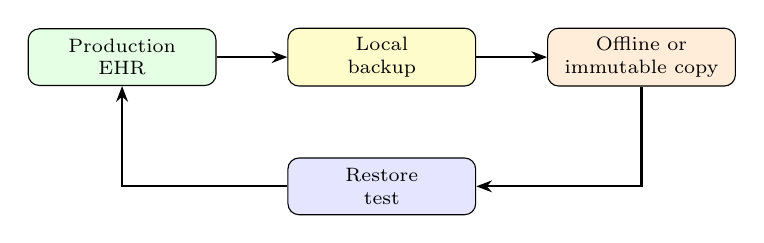
\begin{tikzpicture}[node distance=0.9cm]
\node[opsbox, fill=green!10] (prod) {Production\\EHR};
\node[opsbox, right=of prod, fill=yellow!20] (local) {Local\\backup};
\node[opsbox, right=of local, fill=orange!15] (offsite) {Offline or\\immutable copy};
\node[opsbox, below=of local, fill=blue!10] (restore) {Restore\\test};
\draw[opsarrow] (prod) -- (local);
\draw[opsarrow] (local) -- (offsite);
\draw[opsarrow] (offsite) |- (restore);
\draw[opsarrow] (restore) -| (prod);
\end{tikzpicture}
\end{adjustbox}
\end{center}
\end{frame}

\begin{frame}[c]{RPO and RTO}
\begin{block}{Two recovery questions}
\textbf{Recovery Point Objective} asks how much data loss is tolerable. \textbf{Recovery Time
Objective} asks how long the service can be down before harm becomes unacceptable.
\end{block}

\begin{exampleblock}{Running example}
For appointment reminders, losing one day may be tolerable. For medication administration records,
the acceptable loss and downtime may be much lower.
\end{exampleblock}
\end{frame}

\begin{frame}[c]{Restore Testing}
\begin{block}{The uncomfortable truth}
A backup that has never been restored is only a hope. Restore tests should verify data integrity,
application compatibility, credentials, timing, and clinical usability.
\end{block}

\begin{exampleblock}{Running example}
Restoring a database is not enough if OpenHospital cannot start, lab interfaces cannot reconnect,
or staff do not know which paper forms to use during downtime.
\end{exampleblock}
\end{frame}

\begin{frame}[c]{Downtime Procedures}
\begin{block}{Business continuity}
Recovery is not only technical restoration. Hospitals need downtime forms, manual medication checks,
patient identification procedures, laboratory-result communication paths, and a plan for entering
paper records back into the system after recovery.
\end{block}

\begin{exampleblock}{Running example}
When the EHR is unavailable, \scenario{} moves to preprinted admission forms, direct phone calls for
critical lab values, and a later reconciliation process.
\end{exampleblock}
\end{frame}

\takeawaysframe{
\begin{itemize}
    \item Backups are useful only if restoration works.
    \item Immutable or isolated backups limit ransomware leverage.
    \item Clinical downtime procedures are part of recovery.
\end{itemize}
}{
St. Isidore measures backup quality by restored care, not by backup-job success emails.
}

\section{Incident Response}
\sectiontitleframe{Incident Response}

\begin{frame}[c]{Section Context: Incident Response}
\begin{block}{What we are talking about}
Incident response is the organized process for handling security events before they become larger
harm. NIST incident handling guidance emphasizes preparation, detection and analysis, containment,
eradication, recovery, and lessons learned \cite{nist_ir}.
\end{block}

\begin{exampleblock}{Hospital lens}
During an incident, improvisation is expensive. A prepared response team knows who can disconnect
systems, who talks to clinicians, who preserves evidence, and who informs leadership.
\end{exampleblock}
\end{frame}

\begin{frame}[c]{Incident Response Life Cycle}
\begin{center}
\begin{adjustbox}{max width=\textwidth}
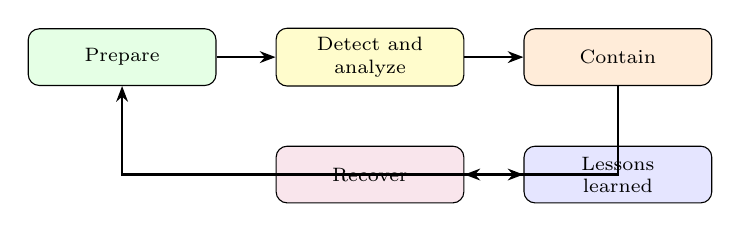
\begin{tikzpicture}[node distance=0.75cm]
\node[opsbox, fill=green!10] (prep) {Prepare};
\node[opsbox, right=of prep, fill=yellow!20] (detect) {Detect and\\analyze};
\node[opsbox, right=of detect, fill=orange!15] (contain) {Contain};
\node[opsbox, below=of detect, fill=purple!10] (recover) {Recover};
\node[opsbox, right=of recover, fill=blue!10] (learn) {Lessons\\learned};
\draw[opsarrow] (prep) -- (detect);
\draw[opsarrow] (detect) -- (contain);
\draw[opsarrow] (contain) |- (recover);
\draw[opsarrow] (recover) -- (learn);
\draw[opsarrow] (learn.west) -| (prep.south);
\end{tikzpicture}
\end{adjustbox}
\end{center}
\end{frame}

\begin{frame}[c]{Prepare Before the Incident}
\begin{block}{Minimum preparation}
Define contacts, roles, escalation paths, legal and privacy contacts, vendor contacts, evidence
handling, emergency procurement, downtime procedures, backup restoration steps, and communication
templates.
\end{block}

\begin{exampleblock}{Running example}
If the EHR is encrypted at 07:20, the hospital should not spend the first hour asking who has the
cloud backup password.
\end{exampleblock}
\end{frame}

\begin{frame}[c]{Detect and Analyze}
\begin{block}{First questions}
What happened? Which systems are affected? Is data encrypted, stolen, or only unavailable? Is the
attack still active? Which clinical services are impacted? What evidence must be preserved?
\end{block}

\begin{exampleblock}{Running example}
The team compares endpoint alerts, proxy logs, authentication logs, file-server events, backup logs,
and staff reports to distinguish malware from an isolated system failure.
\end{exampleblock}
\end{frame}

\begin{frame}[c]{Containment}
\begin{block}{Limit harm}
Containment may include isolating endpoints, disabling compromised accounts, blocking command and
control domains, disconnecting network segments, pausing risky integrations, and preserving backup
copies.
\end{block}

\begin{exampleblock}{Running example}
Disconnecting the laboratory subnet may slow results, but leaving it connected may allow ransomware
to reach analyzers and file shares. The decision must include clinical leadership.
\end{exampleblock}
\end{frame}

\begin{frame}[c]{Eradication and Recovery}
\begin{block}{Return safely}
Remove malware, close exploited paths, rebuild systems when needed, rotate credentials, validate
backups, restore services in priority order, and monitor carefully for reinfection.
\end{block}

\begin{exampleblock}{Running example}
Restoring the EHR before resetting stolen admin credentials may restore the attacker too.
\end{exampleblock}
\end{frame}

\takeawaysframe{
\begin{itemize}
    \item Incident response is planned decision-making under pressure.
    \item Containment decisions must include patient-care impact.
    \item Recovery must avoid reintroducing the attacker.
\end{itemize}
}{
St. Isidore responds as a hospital, not as an isolated IT department.
}

\section{Breach Response and Communication}
\sectiontitleframe{Breach Response and Communication}

\begin{frame}[c]{Section Context: Breach Response}
\begin{block}{What we are talking about}
A security incident becomes a privacy breach when personal data is exposed, lost, altered, accessed
without authorization, or made unavailable in a way that creates risk for people.
\end{block}

\begin{exampleblock}{Hospital lens}
Encrypted file shares may be an availability incident. If attackers also copied patient records, it
is a confidentiality breach. If medication data was corrupted, integrity and safety are involved.
\end{exampleblock}
\end{frame}

\begin{frame}[c]{Breach Triage Questions}
\begin{block}{Assess impact}
Which data was involved? Whose data? Was it encrypted or readable? Was it copied? Could patients
suffer discrimination, fraud, stigma, physical harm, or loss of confidentiality? Which laws,
contracts, or ethics duties apply?
\end{block}

\begin{exampleblock}{Running example}
A leaked appointment list for dermatology is serious. A leaked list for oncology, HIV, psychiatry,
or maternity care may create additional stigma and safety risks.
\end{exampleblock}
\end{frame}

\begin{frame}[c]{Who Needs to Know?}
\small
\begin{tabularx}{\textwidth}{@{}p{0.25\textwidth}X@{}}
\toprule
\textbf{Audience} & \textbf{Communication need} \\
\midrule
Clinical teams & what systems are down, safe workarounds, escalation path \\
Leadership & risk, resources, decisions, legal exposure, patient impact \\
IT and vendors & technical facts, containment, restoration priorities \\
Privacy/legal & breach assessment, notifications, evidence, deadlines \\
Patients & clear facts, risks, support actions, contact point \\
Regulators & required notice, scope, mitigation, follow-up \\
\bottomrule
\end{tabularx}
\end{frame}

\begin{frame}[c]{Incident Communication Principles}
\begin{block}{How to speak}
Communications should be timely, accurate, calm, consistent, and honest about uncertainty. Avoid
speculation, blame, technical jargon, and promises that recovery teams cannot guarantee.
\end{block}

\begin{exampleblock}{Running example}
``We are investigating unauthorized access to some patient records'' is better than ``nothing was
stolen'' before evidence exists.
\end{exampleblock}
\end{frame}

\begin{frame}[c]{Breach Response Scheme}
\begin{center}
\begin{adjustbox}{max width=\textwidth}
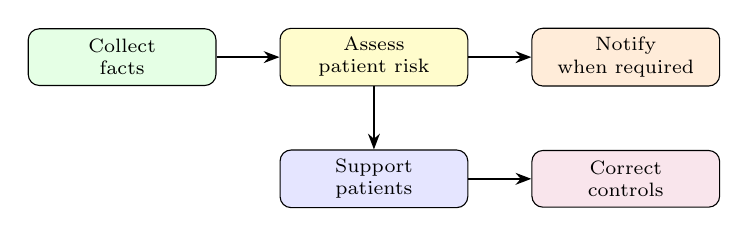
\begin{tikzpicture}[node distance=0.8cm]
\node[opsbox, fill=green!10] (facts) {Collect\\facts};
\node[opsbox, right=of facts, fill=yellow!20] (risk) {Assess\\patient risk};
\node[opsbox, right=of risk, fill=orange!15] (notify) {Notify\\when required};
\node[opsbox, below=of risk, fill=blue!10] (support) {Support\\patients};
\node[opsbox, right=of support, fill=purple!10] (improve) {Correct\\controls};
\draw[opsarrow] (facts) -- (risk);
\draw[opsarrow] (risk) -- (notify);
\draw[opsarrow] (risk) -- (support);
\draw[opsarrow] (support) -- (improve);
\end{tikzpicture}
\end{adjustbox}
\end{center}
\end{frame}

\takeawaysframe{
\begin{itemize}
    \item Breach response is about harm to people, not only harm to servers.
    \item Communication must be coordinated and evidence-based.
    \item Privacy, legal, clinical, and technical teams must work together.
\end{itemize}
}{
St. Isidore communicates to preserve patient safety, trust, and legal accountability.
}

\section{Tabletop Exercise}
\sectiontitleframe{Tabletop Exercise}

\begin{frame}[c]{Section Context: Tabletop Exercise}
\begin{block}{What we are talking about}
A tabletop exercise tests decisions without causing real downtime. Participants walk through a
scenario, identify missing information, make choices, and record improvements.
\end{block}

\begin{exampleblock}{Hospital lens}
The aim is not to embarrass anyone. The aim is to discover gaps before attackers discover them.
\end{exampleblock}
\end{frame}

\begin{frame}[c]{Scenario: Monday 07:20}
\begin{block}{Inject 1}
The emergency department cannot open the EHR. The file server shows ransom notes. A nurse reports
that she opened a spreadsheet called \texttt{urgent\_rota.xlsm}. The laboratory says some results are
delayed.
\end{block}

\begin{exampleblock}{Decision}
Who is incident commander? Which systems are isolated first? What do clinicians do for current
patients? What evidence must not be destroyed?
\end{exampleblock}
\end{frame}

\begin{frame}[c]{Scenario: Monday 08:10}
\begin{block}{Inject 2}
IT finds suspicious admin logins during the night and large outbound transfers from a server. A
local journalist calls reception asking whether patient records were stolen.
\end{block}

\begin{exampleblock}{Decision}
Who speaks externally? What can be said now? Who assesses breach notification duties? Are backups
safe, and who verifies that?
\end{exampleblock}
\end{frame}

\begin{frame}[c]{Scenario: Monday 10:30}
\begin{block}{Inject 3}
Backups exist, but the most recent restore test was eight months ago. The ransom note threatens to
publish oncology and maternity records. Clinical teams are using paper forms.
\end{block}

\begin{exampleblock}{Decision}
Which service is restored first? How are paper records reconciled? How are patients supported if
their data may have been exposed?
\end{exampleblock}
\end{frame}

\begin{frame}[c]{Exercise Output}
\begin{block}{What to produce}
The team should produce an incident timeline, affected systems list, containment decisions, clinical
downtime plan, backup status, communication plan, breach triage, and lessons-learned actions.
\end{block}

\begin{exampleblock}{Running example}
One useful action may be simple: ``test restore every month and document the time needed for EHR,
lab, and file-server recovery.''
\end{exampleblock}
\end{frame}

\takeawaysframe{
\begin{itemize}
    \item Tabletop exercises expose gaps safely.
    \item Decisions must include patient-care priorities.
    \item The output is an improvement plan, not a theatrical performance.
\end{itemize}
}{
St. Isidore practices the day it hopes never arrives.
}

\section{Final Integration}
\sectiontitleframe{Final Integration}

\begin{frame}[c]{Final Concept Map}
\begin{center}
\begin{adjustbox}{max width=\textwidth}
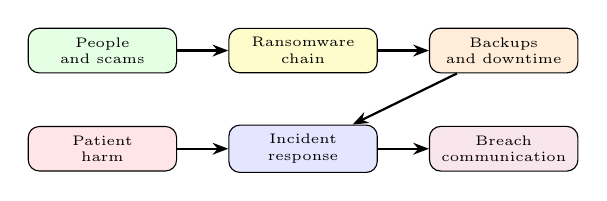
\begin{tikzpicture}[node distance=0.65cm]
\node[smallopsbox, fill=green!10] (people) {People\\and scams};
\node[smallopsbox, right=of people, fill=yellow!20] (ransom) {Ransomware\\chain};
\node[smallopsbox, right=of ransom, fill=orange!15] (backup) {Backups\\and downtime};
\node[smallopsbox, below=of ransom, fill=blue!10] (ir) {Incident\\response};
\node[smallopsbox, right=of ir, fill=purple!10] (breach) {Breach\\communication};
\node[smallopsbox, left=of ir, fill=red!10] (privacy) {Patient\\harm};
\draw[opsarrow] (people) -- (ransom);
\draw[opsarrow] (ransom) -- (backup);
\draw[opsarrow] (backup) -- (ir);
\draw[opsarrow] (ir) -- (breach);
\draw[opsarrow] (privacy) -- (ir);
\end{tikzpicture}
\end{adjustbox}
\end{center}
\end{frame}

\begin{frame}[c]{Final Recap}
\begin{block}{Core lesson}
Operational security is where the course becomes real. Prevention reduces incidents, detection
buys time, response limits damage, backups enable recovery, and communication protects patients and
trust.
\end{block}

\begin{exampleblock}{In \scenario}
\scenario{} cannot promise that incidents will never happen. It can promise preparation: trained
staff, tested backups, segmented networks, useful logs, practiced response, and honest
communication.
\end{exampleblock}
\end{frame}

\begin{frame}[allowframebreaks]{References}
\bibliographystyle{apalike-AMS}
\bibliography{main}
\end{frame}

\end{document}
